\documentclass[11pt]{article}
%Gummi|065|=)
\title{\textbf{CS 374 Spring 2018\\Homework 2}}
\author{Nathaniel Murphy (njmurph3@illinois.edu)\\
		Tanvi Modi (tmodi3@illinois.edu)\\
		Marianne Huang (mhuang46@illinois.edu)}
\date{}

\usepackage{a4wide}
\usepackage{amsmath}
\usepackage{amsthm}
\usepackage{amssymb}
\usepackage{mathtools}
\usepackage{tikz}
\usetikzlibrary{automata,positioning}

\usepackage{enumitem}
\usepackage{scrextend}

\begin{document}

\maketitle
\section*{Problem 1}
Let us first define some functions and notation that will simplify this problem:
\begin{itemize}
	\item Let $s$ be a binary string. Let us indtroduce notation $s_i$, which defines the value of the $i^{th}$ character from the end of the string (zero indexed). i.e. $s=1110,\hspace{1mm}s_0=0,\hspace{1mm}s_1=1$
	\item Define $b_k:2^k\rightarrow\mathcal{P}(\Sigma_k)$ such that for a given binary string $s$ of length $k$,\\$b_k(s)=\{a\in\Sigma_k\hspace{1mm}|\hspace{1mm}s_a=1\}$. Notice that $b_k(s)\subseteq\Sigma_k$.
\end{itemize}

\subsection*{(a)}
Let us define $M=(Q,\Sigma,\delta,s,A)$.
\begin{itemize}
	\item $Q=\{0,1\}\times2^2\cup \{t,g\}$, where $2^2$ is all binary strings of length 2.
	\item $\Sigma=\Sigma_k\cup\{\natural\}=\{0,1\}\cup\{\natural\}$
	\item $s=(0,00)$
	\item $A=\{t\}$
	\item $q$ is defined by the following. Note that for some case3s we use numerical values fo the state names to determine the next state. Also note that $q\in Q=q(i,j)$, where $i\in\{0,1\}$ and $j\in2^2$. Note that we also use $|$ symbol to represent bitwise OR between two binary strings.
	\[\delta(q,a)=\delta\big((i,j),a\big)=\begin{cases}
		(0,j|j') & \text{if } i=0,\hspace{1mm}a\in\{0,1\}, \text{where }j'_a=1,\text{ and all other positions are zeroes}. \\
		(i+1,j) & \text{if }i=1,\hspace{1mm}|j|\geq1\text{ and }a=\natural \\
		t & \text{if }i=1\text{ and }a\in b_k(j) \\
		(1,j) & \text{if }i=1\text{ and }a\notin b_k(j) \\
		g & \text{otherwise}
	\end{cases}\]
\end{itemize}
\newpage \ \\
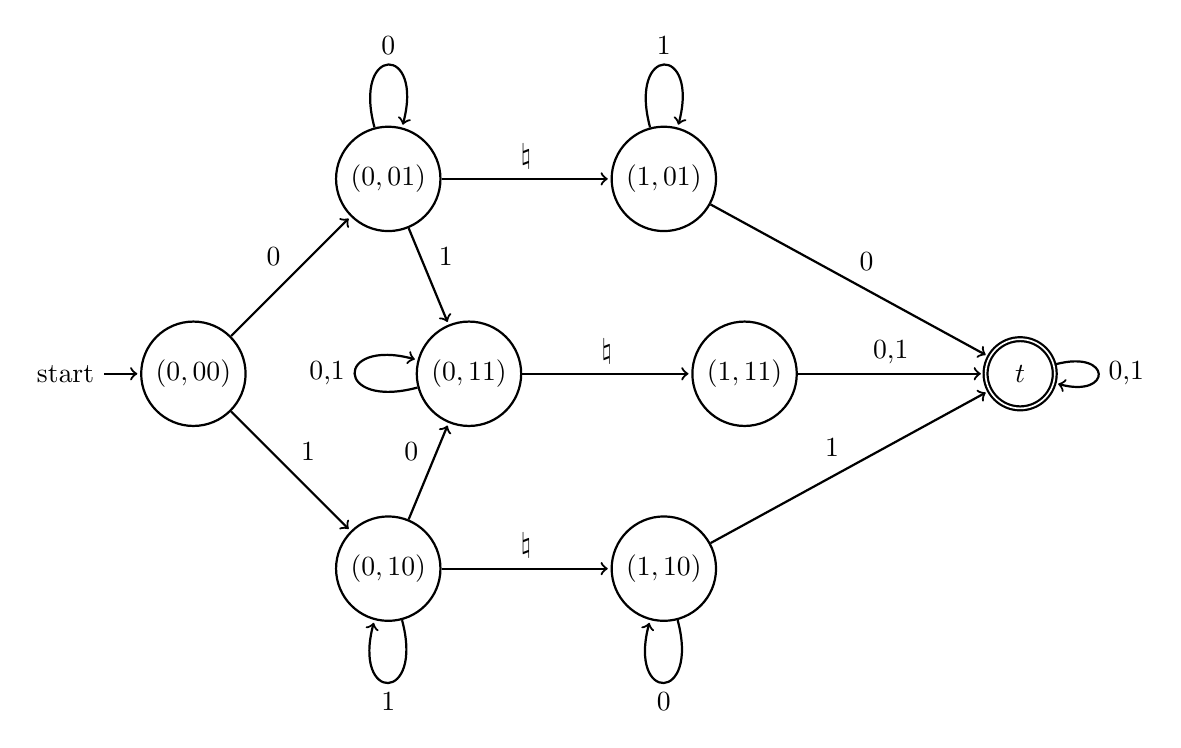
\begin{tikzpicture}[->,shorten >=1pt,auto,on grid,node distance=3.5cm, thick,node/.style={circle,draw}]
	\node[state,initial] (qs) {$(0,00)$};
	\node[state] (q0) [above right=of qs] {$(0,01)$};
	\node[state] (q1) [below right=of qs] {$(0,10)$};
	\node[state] (q2) [right=of qs] {$(0,11)$};
	\node[state] (q3) [right=of q1] {$(1,10)$};
	\node[state] (q4) [right=of q0] {$(1,01)$};
	\node[state] (q5) [right=of q2] {$(1,11)$};
	\node[state,accepting] (qt) [right=of q5] {$t$};
	\path[->]
	(qs)	edge node {0} (q0)
			edge node {1} (q1)
	(q0)	edge [loop above] node {0} ()
			edge node {1} (q2)
			edge node {$\natural$} (q4)
	(q1)	edge [loop below] node {1} ()
			edge node {0} (q2)
			edge node {$\natural$} (q3)
	(q2)	edge [loop left] node {0,1} ()
			edge node {$\natural$} (q5)
	(q3)	edge [loop below] node {0} ()
			edge node {1} (qt)
	(q4)	edge [loop above] node {1} ()
			edge node {0} (qt)
	(q5)	edge node {0,1} (qt)
	(qt)	edge [loop right] node {0,1} ()
	;
\end{tikzpicture}
\newpage \ \\
\subsection*{(b)}
We will prove the following statement by induction on $|w|$. For every string $w$,
\begin{enumerate}[label=\textbf{(\alph*)}]
	\item $\forall\hspace{1mm}w\in\Sigma_k^*,\hspace{1mm}\delta^*(s,w)=(0,j)$ iff $\natural\notin w$ and $w\in b_k(j)^*$
	\item $\forall\hspace{1mm}w\in\Sigma_k^*,\hspace{1mm}\delta^*(s,w)=(1,j)$ iff $w\in\{u\natural v,u\in b_k(j)^*,\hspace{1mm}v\in\Sigma_k^*\cup\{\epsilon\}$ and set$(u)\cap$ set$(v)=\emptyset\}$
	\item $\forall\hspace{1mm}w\in\Sigma_k^*,\hspace{1mm}\delta^*(s,w)=t$ iff $w\in\{u\natural v,\hspace{1mm}u,v\in\Sigma_k^*$ and set$(u)\cap$ set$(v)\neq\emptyset\}$
	\item $\forall\hspace{1mm}w\in\Sigma_k^*,\hspace{1mm}\delta^*(s,w)=g$ iff $w\in\{u\natural v,\hspace{1mm}u,v\in\Sigma_k^*\cup\{\epsilon,\natural\}$ such that either
	\begin{itemize}
		\item $u=\epsilon$
		\item set$(v)\hspace{1mm}\cap$ set$(\{\natural\})\neq\emptyset\}$
	\end{itemize}
	i.e. $w$ starts with a $\natural$ symbol, or contains more than one $\natural$ symbol.
\end{enumerate}
\ \\
We want to prove that all four conditions (a)-(d) hold for every string $w$. \\ \\
\underline{\textbf{Base case}:} $|w|=0,\hspace{1mm}w=\epsilon$. By our definition of $delta$, we see that $delta^*(s,w)=\delta^*(s,\epsilon)=(0,00)$, which is in the form $(0,j)$, where $j=00$. We see that $\natural\notin w$ and $w\in b_k(j)^*$ vacuously. The base case holds. \\ \\
\underline{\textbf{Inductive hypothesis}:} Assume that for any string $w$ of length less than $i$, conditions (a)-(d) hold. \\ \\
\underline{\textbf{Induction Step}:} Consider $w$ of length $i$, where $i>0$. Without loss of generality, we can say that $w=ua$, where $u\in\Sigma^*$ and $a\in\Sigma$. We see that
\[\delta^*\big((0,00),ua\big)=\delta^*\Big(\delta^*\big(0,00),u\big),a\Big)=\delta\Big(\delta^*\big((0,00),u\big),a\Big)\]
Using the inductive assumption, let us prove cases (a)-(d). \\ \\
\underline{\textbf{Case (a)}:} $\delta^*\big((0,00),u\big)=(0,j)\Rightarrow\natural\notin u$ and $u\in b_k(j)^*$ \\
\begin{addmargin}[2em]{0em}
Let us consider all inputs: \\
\underline{$a\in\{0,1\}$:} \\
Then $\delta\Big(\delta^*\big((0,00),u\big),a\Big)=(0,j|j')$, where $j'$ is defined above. This implies that $\delta^*\big(0,00),w\big)$ is still in the form $(0,j)$, which implies that $\natural\notin w$ and $w\in b_k(j)^*$. We see that the first condition ($\natural\notin w$) trivially holds, and that $w\in b_k(j|j')$ by our construction of $j'$.
\newpage \ \\
\underline{$a=\natural$:} \\
We see that if $|u|=0$, $\delta\Big(\delta^*\big((0,00),u\big),\natural\Big)=g$ which implies that $w=ua$ must have a $\natural$ in the first position. this is, in fact the case because $|u|=0$. Let us now assume that $|u|\geq1$. by our definition of $\delta$, $\delta\Big(\delta^*\big((0,00),u\big)\natural\Big)=(1,j)$ such that $u\in b_k(j)^*$. To be in state $(1,j)$, our string $ua=w$ must be in the set
\[L_{(1,j)}=\{u\natural v\hspace{1mm}|\hspace{1mm}u\in b_k(j),v\in\Sigma_k^*\cup\{\epsilon\}\text{ and set}(u)\cap\text{ set}(v)=\emptyset\}\]
By inductive assumption, $u\in b_k(j)\Rightarrow u\natural = u\natural\epsilon=u\natural v\in L_{(1,j)}$ because set$(u)\hspace{1mm}\cap$ set$(v)=$ set$(u)\hspace{1mm}\cap$ set$(\epsilon)=$ set$(u)\hspace{1mm}\cap\emptyset=\emptyset$.
\end{addmargin}
\ \\
\underline{\textbf{Case (b)}:} $\delta\big((0,00),u\big)=(1,j)\Rightarrow u\in\{u'\natural v'\hspace{1mm}|\hspace{1mm}u'\in b_k(j),v'\in\Sigma_k^*\cup\{\epsilon\}$, set$(u')$ $\cap$ set$(v')=\emptyset\}$.
\begin{addmargin}[2em]{0em}
\ \\
Let us consider all inputs: \\
\underline{$a\in\{0,1\}$:} \\
By our definition, if $a\in b_k(j)$, then $\delta\Big(\delta^*\big((0,00),u\big),a\Big)=t$, which implies that $w=ua\in\{u\natural v\hspace{1mm}|\hspace{1mm}u,v\in\Sigma_k^*$, set$(u)$ $\cap$ set$(v)\neq\emptyset\}$. By inductive assumption, $u\in b_k(j)\subseteq\Sigma_k^*$, so $u\in\Sigma_k^*$. We also see that $v\in\Sigma_k^*\cup\{\epsilon\}\Rightarrow v\cdot a\in\Sigma_k^*$ because $\{0,1\}\subset\Sigma_k^*$. It follows that $a\in b_k(j)\Rightarrow$ set$(u)$ $\cap$ set$(v'a)\neq\emptyset$ because $a$ is a common symbol in both strings. \\ \\
\underline{$a=\natural$:} By our definition of $\delta$, if $a=\natural$, then $\delta\Big(\delta^*\big((0,00),u\big),\natural\Big)=g$, which implies that $u\natural$ is in the set $\{u\natural v\hspace{1mm}|\hspace{1mm}u,v\in\Sigma_k^*\cup\{\epsilon\},u=\epsilon$ or set$(v)$ $\cap$ set$(\{\natural\})\neq\emptyset\}$ which means that either $u\natural$ starrts with a $\natural$ or contains more than one $\natural$ symbo. $u\natural$ cannot star5t with a $\natural$ because, by inductive assumption, $u$ does not start with $\natural$ becuase $u$ is in a state with form $(1,j)$. Now, we see that $u\natural$ must contain 2 $\natural$ symbols because, by inductive assumption, $u$ contains one $\natural$ symbol, so $u\natural$ must contain 2 $\natural$ symbols.
\end{addmargin}
\underline{\textbf{Case (c)}:} $\delta^*\big((0,00),u\big)=t\Rightarrow u\in T_k=\{u'\natural v'\hspace{1mm}|\hspace{1mm}u',v'\in\Sigma_k^*$, set$(u')$ $\cap$ set$(v')\neq\emptyset\}$
\begin{addmargin}[2em]{0em}
\ \\
Let us consider all inputs: \\
\underline{$a\in\{0,1\}$:} \\
By inductive assumption, we trivially see that if $a\in\{0,1\}\subseteq\Sigma_k^*,\hspace{1mm}u\in T_k\Rightarrow ua\in T_k$ which agrees with our definition of $\delta:\hspace{1mm}\delta(t,0)=\delta(t,1)=t$. \\\\
\underline{$a=\natural$:} \\
By our definition of $\delta$, $\delta(t,\natural)=g$, so $\delta^*\big((0,00),ua)=\delta\Big(\delta^*\big((0,00),u\big),\natural\Big)=g$. We must now prove that either $w=u\natural$ starts with a $\natural$ symbol or contains 2 $\natural$ symbols. By the inductive assumption, we see that $u=u'\natural v'$ contains one $\natural$ symbol which implies that $u\natural$ contains 2 $\natural$ symbols.
\end{addmargin}
\newpage
\ \\
\underline{\textbf{Case (d)}:} $\delta^*\big((0,00),u\big)=g\Rightarrow u\in L_g=\{u'\natural v'\hspace{1mm}|\hspace{1mm}u',v'\in\Sigma_k^*\cup\{\epsilon,\natural\},$ set$(v')$ $\cap$ set$(\{\natural\})\neq\emptyset\}$
\begin{addmargin}[2em]{0em}
\ \\
Let us consider all inputs: \\
\underline{$a\in\{0,1,\natural\}$:} \\
$\delta(g,a)=g\Rightarrow]\delta\Big(\delta^*\big((0,00),u\big),a\Big)=g$. It is trivial to show that $u\in L_g\Rightarrow ua\in L_g$ because $u=u'\natural v'\Rightarrow ua=u'\natural v'a=u'\natural v$ holds because $a\in\Sigma_k^*\cup \{\epsilon,\natural\}$ and set$(v')$ $\cap$ set$(\{\natural\})\neq\emptyset\Rightarrow$ set$(v'a)$ $\cap$ set$(\{\natural\})\neq\emptyset$. \\ \qed
\end{addmargin}
\end{document}
